You can write monospace letters \texttt{like that}.

You can create itemization like that:
\begin{itemize}
	\item Example item 1
	\item Example item 2
	\begin{itemize}
		\item Example subitem 1
		\item Example subitem 2
	\end{itemize}
	\item Example item 3
\end{itemize}

You can cite like that:
\cite{torvalds2001just}
\cite{kopka2004guide}
\cite{yakaryilmaz2011unbounded}
\cite{bernstein2019fast}

If you need to give a page number, you can cite like that:
\autocite[11]{almheiri2021entropy}

You can create a table like that:
\begin{table}[ht]
	\caption{An Example Table}
	\begin{center}
		\begin{tabular}{|c||c|c|}
			\hline
			Example 1.1 & Example 2.1 & Example 3.1 \\
			\hline
			Example 2.1 & Example 2.2 & Example 2.3 \\
			\hline
		\end{tabular}
	\end{center}
	\label{tab:example}
\end{table}
Also, you can refere a table like that: "Table \ref{tab:example}".

\blindtext[1]

You can create a figure like that:
\begin{figure}[ht]
	\begin{center}
		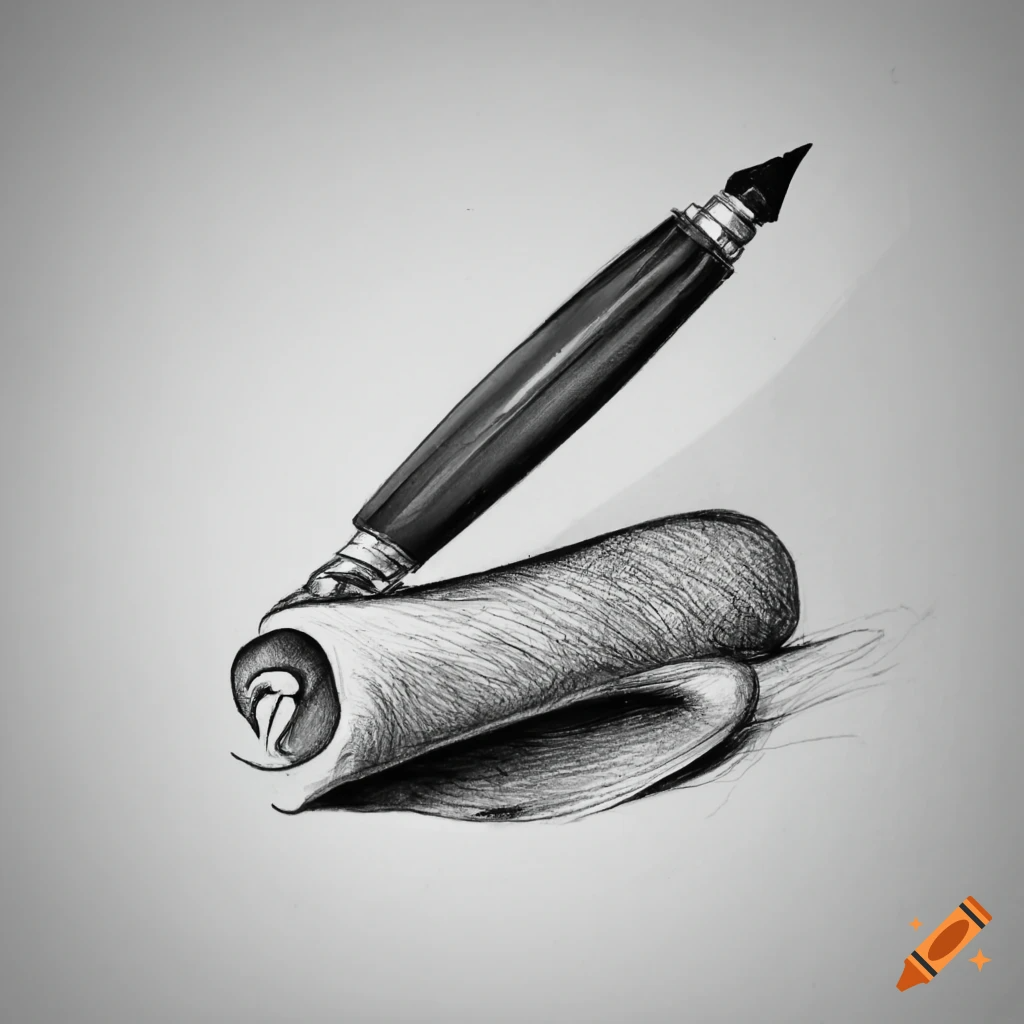
\includegraphics[scale=0.2]{chapters/images/example-figure.png}
	\end{center}
	\caption{An Example Figure}
	\label{fig:example}
\end{figure}
Also, you can refere a figure like that: "Figure \ref{fig:example}".

\blindtext[1]